\chapter{Introduction and Background information}
\section{Motivation}
\label{sec:Motivation}
The motivation of this thesis is to show the methodology that can be used both by applied researchers and clinicians to draw meaningful survival inference from data with a high amount of missingness. While both fields are well studied, their interaction is not. I want the methods  to be easy enough to describe to someone with a limited statistical background, but meaningful and valid so that the results obtained can be used in publication. The desire to have it this way stems from working on a related project with both statisticians and clinicians. While we will be motivated by cancer data, I believe that the methods used in this thesis are general enough to be applied to other types of survival data.

\label{ch:Intro}
Missing data is a major problem in both statistics and medicine, however, it has not received attention proportional to its need. Survival analysis is well studied, but is relatively complete, so not much new research comes out of this field. Propensity score analysis will help us determine causal relationships when we don�t have a completely randomized experiment. As one could imagine, all three of these fields are important to the applied statistician, as they will come across at least one at some point in their career.  The goal of this thesis is to demonstrate how to use all three in trio, a topic that has only received little interest in the literature. I will explain each of these three disciplines in detail before we dive into combining them.

\section{Imputation}
\label{sec:Imputation}
In an ideal world, we would have complete data with no missingness, however this is rarely ever the case. Imputation (specifically multiple imputation) is a way to �fill in missing data� with plausible values, and it forms the base of this paper. All of the other analyses that will be used will follow from it, thus we need a good understanding of it before we may proceed. Imputation itself has been around since the 1970�s, but multiple imputation is a recent development, proposed formally in 1987 by Donald Rubin \cite{Rubin1987}. To understand the use and importance of multiple imputation, we need to understand the problem of missing data, and the previous attempts to deal with it.

At first, statisticians payed no attention to missing data, and happily discarded records for their analysis that were incomplete. This procedure is known as complete case analysis. There are many problems with this paradigm. To begin with, you will lose a lot of statistical power when doing this, because you are literally throwing away records and thus decreasing your sample size.  In addition, this can be costly to the researcher. If it costs a set amount to collect a single record, and you don�t use this record, you are literally wasting money. As well, in some rare cases, incomplete data might be the only type we can get (like if we have a machine that analyzes a blood sample chemical level, but can�t detect it if the level is too high or low). Lastly, and most importantly, we will be biasing our estimates if we discard them. For example, if we have a random sample of people and are testing a drug, and want to run a regression on some collected covariates. Men are known to not want to give all of their information, so they leave them blank. In the analysis, we will need to discard the male samples because they are incomplete, leaving us only with women. Thus, we don�t have a random sample anymore, and will get biased results because we have knowingly thrown away half of our data which we know to be different.

A slight improvement on this is called available case analysis. In this setting, a record is used in the analysis if it has all of the needed information for that analysis. So, a record could have missingness, but if the covariate with missingness is never used in the analysis, it will not be discarded. This paradigm is the standard analysis type for most statistical packages. It is better than complete case analysis, but is still flawed. We are still throwing away valuable data as we were with complete case analysis, although likely not as much. Available case analysis will still lead to bias in the same way that complete case did too. As well, new complications arise in available case analysis, namely that nonsensical situations like correlations outside of $\pm 1$, and inconsistent sample sizes for different analyses can arrise.

The next wave of statisticians wanted to improve upon available case analysis, so they developed what we now call today imputation. Their specific incarnation was called single imputation, and their goal was to fill in missing values with a plausible replacement value. A single method (such as regression, taking the mean, resampling) is used one time to impute the missing value. While this is a little better than complete case analysis, it still has many drawbacks. Asserting that a single value is the true value is unjustified and foolish. There is always some amount of error  and uncertainty involved, and we can in no way be 100\% confident that our imputed value is correct. Furthermore, if I impute one value and you impute another, we may get totally different results from analysis on the data. This is obviously not a desirable trait.  In addition, imputing one time and calling it your data will artificially increase your sample size. You are in effect treating the imputed values as if they were real, inflating your sample size with data that was not actually observed. This will give you unjustified statistical power and accuracy. While single imputation certainly has its drawbacks, the idea of actually trying to fill in the data is an important one, and multiple imputation fills in the gaps that single imputation is not able to cover.
\begin{comment}
\begin{figure}[h!]
  \caption{Visualization of MI data}
  \centering
    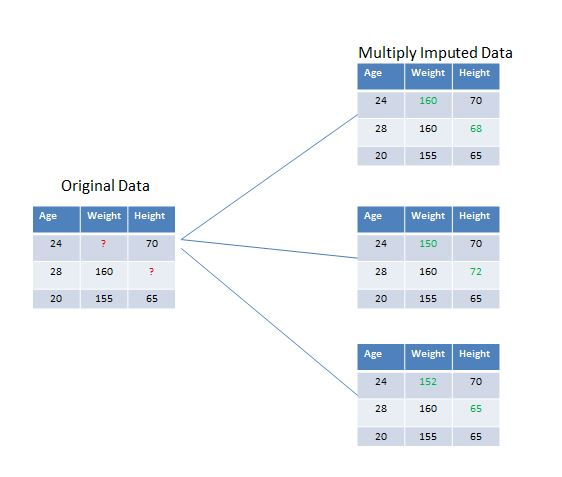
\includegraphics{mi_example.jpg}
\end{figure}
\end{comment}
Multiple imputation began in the 1970�s, but it wasn�t until 1987 when the Donald Rubin formalized multiple imputation methodology in his seminal book� multiple imputation for nonresponse in survey� did it start to gain acceptance \cite{Rubin1987}. The central idea is to frame the problem in a Bayesian framework, and produce $m\geq 2$ values to substitute in for each missing value, drawing these values from the missing covariates posterior distribution. Using these substitute values (m values), we can think of the data now as being m datasets, each dataset having the observed data, and one value of the missing data. This might be hard to think about, but seeing a visualization of it will make it clear !! put in figure here!! . Once we have a sufficient number of datasets (we will talk about how to pick the number later), we can run whatever analyses we would like on them individually, treating the dataset as if it was complete. Once we have run the model on the $m$ datasets, we can pool the results to get one estimate. We can get the standard errors by noting the within and between imputation variance. 

This method is obviously much better than the first two methods because it allows is to not throw away data, as well as allowing us to quantify our uncertainty about imputing the missing values. The only real drawback of multiple imputation is that we still don�t have true data, but we can be confident enough in our estimations to compensate for that. The use of multiple imputation has been steadily increasing over the past 30 years, and it is now the standard for missing data. Stef van Burren, an influential author in multiple imputation did a study of academic papers, and concluded that the number of publications using or mentioning multiple imputation is growing at an exponential rate since about 1990 \cite{VanBuuren2012}.



\section{Survival}
\label{sec:Survival}
Survival analysis is a huge field, and there have been many textbooks written about it. I only plan to introduce the topics that are relevant to my case study.  For a much more detailed account of survival analysis, please see \cite{Klein1984}.
Survival analysis on the whole can generally be described as the analysis of time to event data, often in the presence of censoring (when we don�t have complete information about the time of failure).  There are many techniques used in this field, but the main tools that we will be using are Kaplan-Meier estimates, log rank tests, and Cox regression. 

Before we go on, it should be noted that often in the literature (and in this paper), we see terms like �death� and �survivors�. This is due to survival analysis being heavily intertwined with medical studies. A more general term for these would be �event� and �those who have not had an event yet�. You don�t actually have to die to be considered a death, you just need to have had the event of interest. Survival analysis doesn�t have to be gloomy!

The Kaplan-Meier estimator (sometimes called the product limit estimator) is a non-parametric estimate of the true survival function (the probability that you survive after time t).  It is defined as 
$$\hat{S}(t)=\prod_{t_i<t}\frac{n_i-d_i}{n_i}$$
Where $n_i$ is the number of �survivors� minus the number of censored cases just prior to time $t_i$, and $d_i$ is the number of deaths or events that you observe at time $t_i$. The Kaplan-Meier estimator is very commonly used as a measure to see how different treatments affect survival time
The log-rank test is a popular nonparametric test that researchers often use to see if two or more survival curves come from the same distribution. This is a useful tool to have, because visualizing curves alone does not give us this information (we could have two curves that look radically different due to sampling error, yet still come from the same distribution). Knowing about if the survival curves come from the same or different distribution is useful because it allows us to make statements like �drug a is associated with longer survival time than drug b�. It is given by
$$\frac{\sum_{j=1}^{J}(O_{1j}-E_{1j})}{\sqrt{\sum_{j=1}^{j}V_{j}}}\sim N(0,1)$$
!!! Work on this more, put the definitions!!
This test as it is places equal weight to all of the deaths we observe, although there are other formulations of this test that give more weight to early or late deaths. This is useful for example if we have a drug that is supposed to improve your life expecentacy, we wouldn�t care about early deaths , only about later times. Putting more weight on the later deaths would help to answer this question.
It can be proven that the log-rank test is equivalent to the score test on a cox model of the same data with no ties \cite{Klein1984}. We will speak about the Cox model next.

Proportional hazards regression, often called Cox regression is a modelling tool that allows us to analyze the hazard ratio of a covariate, assuming that each covariate acts to multiply the hazard ratio. The hazard is a survival tool that tells us the rate of events at time t, conditional on survivorship until time t. Mathematically, it is given by
$$h(x)=\lim_{\Delta x\rightarrow0}\frac{P[x\leq X<x+\Delta x|X\geq x]}{\Delta x}$$
  Cox regression is a maximum likelihood method estimator, given by 1
$$h(t|Z)=h_{0}(t)\exp(\sum_{k=1}^{p}\beta_{k}Z_{k})$$
The $h_0(t)$ is what�s known as the baseline hazard, and can be any function that we would like. We aim to maximize the betas with respect to the partial likelihood. Our inference of interest is 
$\frac{h(t|Z)}{h(t|Z^{*})}=\exp(\sum_{k=1}^{p}\beta_{k}(Z_{k}-Z_{k}^{*}))$
Where Z* is another set of covariates. The relative risk (or hazard ratio) describes the relative risk of two subjects with two different covariates. This ratio will be a constant, hence the name proportional hazards, and does not depend on the baseline hazard.

Using cox regression, we can make statements such as   �increasing the drug by one mg will increase its hazard by 30\%�. 

<<!!! Maybe put something here about competing risks if we want to do that!!
\section{Propensity Score Analysis}
\label{sec:PSA}
<<THIS NEEDS A LOT MORE WORK>>
Observing data is good, but unless we conduct a completely randomized experiment, we cannot make any claims about causality. In an ideal world we would like to be able to do research and say that A causes B, not something along the lines of �our study says that A is associated to B�.  

We are not out of luck though, because by using Rubin�s causal model, we can talk about causation in this setting. Our goal is to determine the causal effect of a treatment.  To do so, we need to have a completely randomized experiment, where the differences in the groups outcome can only be attributed to the differences in the treatment. When we have a non randomized experiment, we incur bias, because differences can come from things besides the treatment. Under Rubin�s causal model, we aim to balance the groups out so that it is like there was random assignment. Our ultimate goal is to look at each subject and see how they react to the treatment and to the control. This is obviously impossible, since a person cannot at the same time take the treatment and control. This is what�s called the fundamental problem of causal inference. We can only observe one outcome and that is the issue. We need what is known as the counterfactual, or the other potential outcome. We go about getting this by matching a subject with a set of covariates to someone who is very similar from the other group. We then look at all of the subjects differences to see if there truly is a causal effect.

The way we will match is on the �propensity for treatment�, or simply propensity score. This is often done by logistic regression, although newer methods include regression trees and other binary classifiers.  Its use is justified by the propensity score theorem, which states that if we assume conditional independence of the treatment given covariates on the outcomes, then we can also assume conditional independence of the treatment given the propensity score on the outcomes. Symbolically
$$(Y(0),Y(1))\perp T|X\implies(Y(0),Y(1))\perp T|p(X)$$

The proof can be found in\cite{Angrist2008}. So, now we have the probability or propensity of a subject being assigned to a specific treatment given their covariates, even if they were not actually assigned to that treatment. What this says is that we can now match on a single number (the propensity score), rather than match on many covariates. We can now match each on their propensity scores. Once we have our groups, we can examine the average causal effects, and do causal inference.
